\section{Problem Definition}
\label{sec:problem}

%In this section, we first give formal definitions of the knowledge base
%and the schema graph, then describe the paraphrasing task.

\begin{definition}
A {\em Knowledge Base} is a triple $\langle E, L, P\rangle$, where:
$E$ is a finite set of all entities in $KB$;
%$T$ is a finite set of all types in $KB$;
$L$ is a finite set of all predicate names in $KB$;
%  All the entities, types and predicate names in $KB$ are identified by a unique id.
$P$ is a finite set of predicate instances with the form
$p(e_1, e_2)$ where $e_1, e_2 \in E$ and $p \in L$.\footnote{A special
type of predicate in many knowledge bases is ``IsA'', which connects an
entity with its {\em type}. However, for simplicity we treat a type as a
special entity.}
%$IsA$ is the special isA relation, with the form $isa(e, t)$;
%and each entity has at least one type.
\end{definition}

%\KQ{Add some sentences showing what's a schema: abstraction}

%1. relation comes from a detail subgraph (give an example of mo_of)
%A knowledge base is capable of representing complex relations
%between real entities.
%As what we've shown in \figref{fig:fb-schema}, though there is no
%direct grandfather relation between ``Pactrick Schwarzenegger''
%and ``Gustav Schwarzenegger'', they can be indirectly connected via
%the ``parent + parent + male'' structure.
%2. relation schema is a summarization o a list of subgraphs. (by substitution)
%Intuitively, different instances of a complex relation type share a
%common structure (the schema), which is the template of that relation.
%Now we give the formal definition of a schema graph.

%3. formal def. of S
\begin{definition}
A \textit{Schema} (denoted by $S$), is a triple
$\langle E', X, P_S \rangle$ where:
  $E' \subseteq E$, i.e.,
  a subset of entities in KB respectively;
  $X$ is a finite set of different variable entities, and  each $x \in X$
  indicates a placeholder for an entity $e \in E$;
  two special variables in $X$, $x_{subj}$ and $x_{obj}$, denote the
  subject and object entity of the relation respectively;
  %\item $C=\{\text{solid, dashed, isa}\}$, representing 3 different
  %category labels of predicates in $S$.
  $P_S$ is a finite set of \textit{schema predicate instances} as
  $p_s(v_1, v_2)$ where $v_1 \in X$, $v_2 \in E' \cup X$
  and $p_s \in L$. Moreover,
\begin{itemize}
  \itemsep0em
  \item $S$ represents a directed tree structure, the root of which is
the subject entity $x_{subj}$;
  \item the path between $x_{subj}$  to $x_{obj}$ in the schema is called
	the {\em skeleton} of the schema;
  \item all edges other than the skeleton are called {\em constraints};
  \item a schema with only a skeleton and no other edges, is called
	 skeleton schema, or skeleton in short.
%   \KZ{How do you ensure that
%	all nodes internal nodes are variables and all external nodes are
%	are constants or $x_1$ or $x_2$. Also how do we say that there's no
%	two consecutive variable nodes in the tree. These are not clear now.}
%  \item On the path from $x_1$ to $x_2$ (which is the skeleton
%        of $S$), all vertices $v \in X$.
%  \item In the tree, all non-leaf vertices $v \in X$.
%  \item[-] $c = \text{solid}$, if and only if $v_1, v_2 \in X$, $p_s \in L$,
%  \item[-] $c = \text{dashed}$, if and only if $v_1 \in X, v_2 \in E'$, $p_s \in L$,
%  \item[-] $c = \text{isa}$, if and only if $v_1 \in X, v_2 \in T'$ and $p_s = \text{isa}$.
\end{itemize}
%\KZ{I think the input $e_1$ and $e_2$ should be separated from E'. These
%are the target entities, different from other concrete entities in the
%schema.}
  %These restrictions make every predicate in $S$ connecting to at least one variable.
  %Generalize the definition. We do not need the graph to be a tree.

  %\item[*] All $solid$ predicates form a tree, where both $x_{subj}$ and $x_{obj}$ must
  %be a leaf, that is, linked by only one $solid$ predicate.
\end{definition}
\figref{fig:schema-example} shows a general style of a schema graph.
Note that every edge of the graph must connect at least one variable entity.
%4. a small sentence describing the relation between S, G and hits.
A \textit{ground graph} is a subgraph of $KB$ that is
instantiated from a relation schema $S$, with
every variable $x_i$ instantiated with entity $e_i \in E$.
%Take ``starringIn'' schema in \figref{fig:fb-schema}(c) as an example,
%one of its ground graphs in Freebase is shown in \figref{fig:ground-graph}.
If a ground graph of $S$ instantiates $x_{subj}$ to $e_{subj}$ and $x_{obj}$ to
$e_{obj}$, then $S$ is said to {\em cover} the entity pair $(e_{subj}, e_{obj})$.
%And we define the \textit{coverage} of $S$ as all entity pairs covered by it in $KB$.
%Combining together all ground graphs of a schema,
%we can define the \textit{hit pairs} of a schema:

%5. formal def. of Hits. (S, G1, G2, ... ==> HP(S))
%\begin{definition}
%\textit{Hit Pairs}. Let $S$ be a schema and $G$ be a ground graph of $S$. The entity pair $\langle e_1, e_2 \rangle$
%is a $hit$ of $S$. \KZ{What is $e_1$ and $e_2$? They are actually the input
%entity of the schema. This is not clear here.}
%In addition, $HP(S)$ is the \textit{hit pairs} of $S$,
%which is a set of all hits derived from the ground graphs of $S$.
%\end{definition}

\begin{figure}[t]
\centering
%\epsfig{file=fb-schema-4.eps, width=0.95\columnwidth}
\scalebox{0.6}{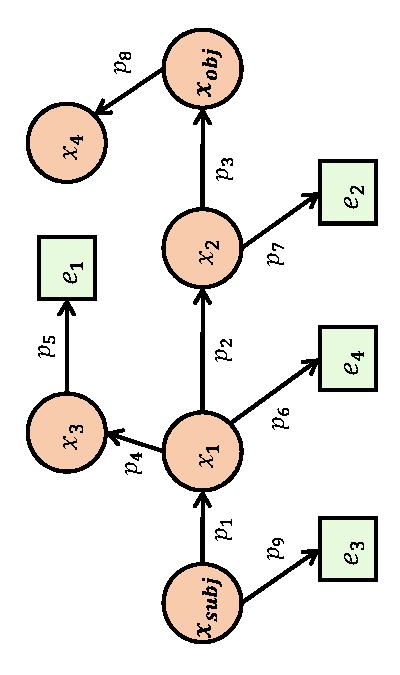
\includegraphics[angle=0]{schema-example-crop.eps}}
\caption{A general style of a schema graph.}
\label{fig:schema-example}
\end{figure}

%\KQ{Put example $S$ here, one for running example, another one for the most simple
%schema covering $|E|^2$ entity pairs.}
%
%A ground graph $G$ is generated from its underlying relation schema $S$, where
%each variable $x$ is instantiated with an entity $e_x \in E$, such that:
%\begin{itemize}
%  \item[-] $\forall p_s(x_1, x_2, \text{solid}) \in P_S,~ p_s(e_{x_1}, e_{x_2}) \in P$,
%  \item[-] $\forall p_s(x, e, \text{dashed}) \in P_S,~ p_s(e_x, e) \in P$,
%  \item[-] $\forall p_s(x, t, \text{ida\_dashed}) \in P_S,~ t \in IsA(e_x)$.
%\end{itemize}
%\noindent
%Actually $G$ is a subgraph of $KB$ with the position of subject and object specified.
%We call the entity pair $\langle e_{subj}, e_{obj} \rangle$ a hit of $G$ and its underlying $S$.
%Grouping each $G$ derived from $S$, we define $HP(S)$ as the set of all hits of $S$.

%1. task is ...

Our problem is, given the $KB$, a natural language relation $r$ along with a set of
instances \{($e_{subj}$, $r$, $e_{obj}$)\}, induce a list of schemas and 
the probability distribution over the schemas, such that observed instances
can be produced with the highest probability.

%find a ranked list of schemas that have the most similar meaning
%to $r$. \KZ{Why isn't the problem one that finds a list of schemas
%that {\em collectively cover} as many input pairs as possible?}

%The weight of each schema represents the fitness score over inputs.
%Intuitively, schema fits input entity pairs properly, if neither too general
%(producing too many coverages),
%nor too specific (only covers a few positive pairs).

%It's clear that output schemas could be selected from any schema covered at least one entity pair.
%However, existing knowledge base could have millions of entities and thousands of different
%kinds of predicates, leading to a huge search space.
%The searching direction is crucial for finding more suitable schemas within
%limit time and space.
%In addition, with no labeled schemas as training data, we need a
%data-driven metric to label each schema with a ``silver'' score, measuring
%the quality of one candidate schema.
%Therefore, we define a function $cost(EP, S)$, measuring the cost of one schema $S$
%with respect to positive input pairs $EP$, and then perform a local search algorithm guided by this function.
%\KZ{Shall we give a more formal def of the paraphrasing problem? You can
%refer to the way it's defined in Gong yu's paper. It's similar.}

%Next, we present an overview of the framework (\secref{sec:approach}),
%and explain how candidate schemas are generated (\secref{sec:candgen}),
%and how the schema probability is computed based on relation instances (\secref{sec:schema}).
%

%and how the silver score is computed to train the classifier for
%schema inference.

%how we obtain the cost function based on the view of information theory (\secref{sec:scoring}),
%and how the local searching process is performed (\secref{sec:candidate}).

%In section 3, we focus on how we build th   based on the view of information theory.
%
%For the local searching algorithm,
%
%Output schemas are chosen from a set of \textit{candidate schemas} in KB,
%which are the most suitable (neither too general nor too specific) for the given data.
%
%In order to describe all given entity pairs, the hit pairs of output schemas
%must cover all the given entities.
%Furthermore, we build a cost function to measure the fitness score over a schema and entity pairs,
%turning our task to an optimization problem.
%%2. bridge the gap bet. entity and schema. that's assign
%%A ground graph bridges the gap between $\langle e_{subj}, e_{obj} \rangle$ and a schema.
%%All schemas that can hit at least one entity pair form the schema searching space.
%%Each entity pair is assigned to at least one schema which hits the pair.
%%After the step of assignment, a cost is produced when a schema is selected
%%to describe all its assigned entity pairs assigned.
%%%3. Goal: Min Cost
%%With cost function provided, we look for a set of schemas describing
%%all entity pairs at a minimum cost.
%
%%4. Formally Define.
%The following is the formal definition of our task.
%
%\begin{definition}[The Paraphrasing Problem]
%\label{def:pp}
%Given $KB$, entity pairs $EP = \{ep_1, ..., ep_n\}$,
%a cost function $f: EP \times S \rightarrow [0, +\infty)$,
%and a function $sel$ that selects all candidate schemas ($CS$) from $KB$,
%return a set of output schemas $OS \subseteq CS$, such that:
%\begin{itemize}
%    \item[-] $EP \subseteq \bigcup_{S \in OS} HP(S)$,
%    \item[-] Whole cost $Z = \sum\nolimits_{S \in OS} f(EP, S)$ is minimum.
%\end{itemize}
%%
%%Given $KB$, a binary relation pattern $rel$ with its support entity pairs
%%$EP = \{ ep_1, ..., ep_n \}$, cost function $f$ and $g$,
%%Let $CS = \{S | EP \cap HP(S) \neq \emptyset \}$ be \textit{candidate schemas} and
%%$DS = \{S_1, ..., S_m\} \subseteq CS$ be a set of \textit{selected schemas}.
%%Let $Ass_{m \times n}$ be an 0/1 \textit{assignment matrix} from $EP$ to $DS$ and
%%\textit{support set} $sup(S_j) = \{ep_i | Ass_{ij} = 1\}$ be all entity pairs assigned to the $j$-th schema.
%%The assignment $Ass$ is a valid assignment over $EP$ and $SG$ if it satisfies the following
%%constraints:
%%\begin{itemize}
%%    \item[-] $Ass_{ij} = 1 \Rightarrow ep_i \in HP(S_j)$,
%%    \item[-] $\forall ep_i \in EP, \exists S_j \in DS, Ass_{ij} = 1$,
%%    \item[-] $\forall S_j \in DS, \exists ep_i \in EP, Ass_{ij} = 1$,
%%\end{itemize}
%\end{definition}
%
%%The selected schemas $DS$ and corresponding $Ass$ are optimal, if it minimizes
%%the cost $Z(DS, Ass) = \sum\nolimits_{S \in DS} f(S) + g(S, sup(S))$ , where $f$ is a
%%cost function over a specific schema, and $g$ is a cost function over a schema along
%%with its support set. Both $f$ and $g$ are non-negative functions and defined by users.
%
%%Now we define the task of paraphrasing between NL and KB. Given KB, a binary relation
%%pattern $rel$ with its support entity pairs
%%$EP = \{\langle e_1^{(1)}, e_2^{(1)} \rangle , ..., \langle e_1^{(n)}, e_2^{(n)} \rangle \}$
%%from KB, we want to find a set of relation schemas $\vec{S}$ that:
%%
%%\begin{itemize}
%%    \item[-] Each entity pair is hit by at least one schema in $\vec{S}$,
%%    \item[-] The schemas fits $EP$ at the best (neither too general nor too specific).
%%\end{itemize}
%%
%%where the score of fitness is produced by a cost function $Cost(EP, \vec{S})$.
%%The cost function captures both compactness and precision for the set of schemas to describe the entity pairs.
%
%
%%\KQ{The reason of restricting at most K relation schemas is to avoid generating too many schemas.
%%In the formula, Cost(EP|S) is the dominant one,
%%probably 5~10 pairs hit by one specific schema could bring that schema into description set.}
%%
%%Next, we prove that the paraphrasing problem is NP-Hard.
%%We show that by constraining $sel$ and $f$ to some specific classes of
%%functions, the resulting instance of the paraphrasing problem can
%%be reduced from the well-known {\em weighted set cover problem},
%%which is NP-complete.
%%
%%\begin{theorem}
%%Given $KB$, $EP$, candidate selecting function $sel$ and cost function $f$,
%%computing the optimal output schemas for describing all pairs in $EP$, is NP-Hard.
%%\end{theorem}
%%
%%\begin{proof}
%%%Rephrase that a simplified instance of our problem is still NP-Hard.
%%We first state the simplified instance of the paraphrasing problem.
%%The function $sel$ is restricted by only returning a special kind
%%of schema, which has only $x_{subj}$ and $x_{obj}$ connected by a solid
%%predicate. In addition, the cost function $f$ is simplified as
%%$g: S \rightarrow [0, \infty)$, that is,
%%the cost is only determined by the schema, and not by EP.
%%
%%After the simplification, the \textbf{decision version} of the
%%paraphrasing problem is as follows:
%%Given $KB$, $EP$, $sel$, $g$ and a threshold $\theta$, is there a set of output schema $OS$
%%covering all pairs in $EP$, such that whole cost $Z \leq \theta$ ?
%%The proof relies on a reduction from \textsc{Weighted Set Cover} problem:
%%Given a universe $U = \{u_1, ..., u_n\}$, a threshold $\theta$, a set $V = \{v_1, ..., v_m\}$
%%whose union equals to $U$, each $v_j \subseteq U$ and a weight set $W = \{w_1, ..., w_m\}$ assigned to each $v_j$,
%%is there a cover $C \subseteq V$ whose union equals to $U$, and the summation weight is no larger than $\theta$ ?
%%
%%\textit{Reduction:} For an arbitrary instance of \textsc{Weighted Set Cover} problem,
%%we build a $KB$ based on $U$ and $V$, where it contains only $m$ different predicates $p_1, ..., p_m$,
%%leading to a set $m$ simple candidate schemas.
%%We map each $u_i$ to an entity pair $ep_i = \langle e_{subj}^{(i)}, e_{obj}^{(i)} \rangle $.
%%For any $u_i$ and $v_j$, if $u_i \in v_j$, we add a predicate instance $p_i(e_{subj}^{(i)}, e_{obj}^{(i)})$ into $KB$.
%%Finally, we define the cost function as $g(S_j) = w_j$ for each schema.
%%
%%Since all schemas have only one edge, retrieving candidate schemas from $KB$
%%along with hit pairs can be done in polynomial time. Therefore, the paraphrasing decision problem
%%is formulated as: Given $n$ entity pairs and $m$ sets of hit pairs whose union cover all pairs,
%%with the weight $w_j$ assigned to the $j$-th set, can I pick some sets that still cover all
%%the entity pairs, satisfying the summation weight no larger than $\theta$ ?
%%Obviously, solving this paraphrasing decision problem is equivalent to
%%solving the corresponding \textsc{Weighted Set Cover} problem.
%%\end{proof}
%%
%%%In this reduction, $U$ and $V$ are used to construct a $KB$,
%%%where $m$ different predicates $p_1, ..., p_m$ are in $KB$,
%%%each $u_i$ indicates an entity pair $\langle e_1^{(i)}, e_2^{(i)} \rangle $,
%%%and the relation instance $p_i(e_1^{(i)}, e_2^{(i)})$ is contained (or not) in $KB$
%%%according to whether $u_i$ is covered by $S_j$.
%%%Since we only consider the schema with one solid edge,
%%%the complexity of finding all \textit{candidate schemas} of these $n$ entity pairs
%%%is within polynomial time, where the $j$-th candidate schema hits those corresponding entity pairs within $V_j$,
%%%with the cost function $f(S_j) = w_j$.
%%%In addition, since the function $g$ is always zero, the assignment step could be ignored (if $S_j$ is selected,
%%%then all its hitting pairs would be assigned it without bringing extra costs).
%%%Therefore, if there exists a cover $C$ satisfying the $\theta$ limit, then
%%%it's possible to select schemas covering all entity pairs with cost no more than $\theta$.
